\section{Amplitude responses of windows} \label{appD}
The figures below show the amplitude responses in dB of the different windows considered for the STFT in section \ref{sec:STFT_variation}.

\begin{figure}[H]
\centering
\begin{subfigure}{0.49\textwidth}
\centering
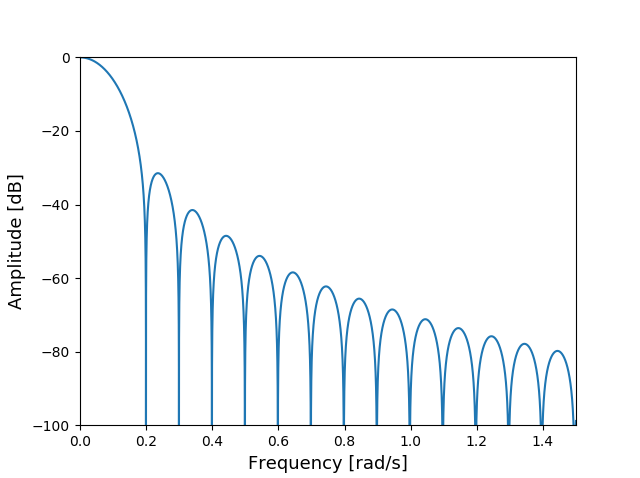
\includegraphics[width=\textwidth]{figures/dbplots/stft_bilag/64/hann.png}
\caption{Hann window.}
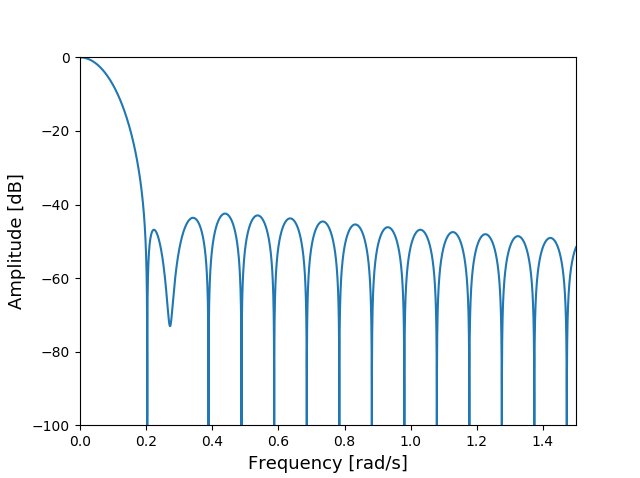
\includegraphics[width=\textwidth]{figures/dbplots/stft_bilag/64/hamming.png}
\caption{Hamming window.}
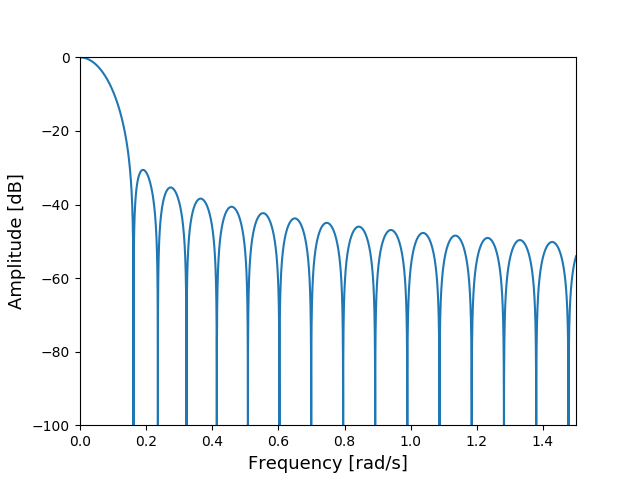
\includegraphics[width=\textwidth]{figures/dbplots/stft_bilag/64/kaiser4.png}
\caption{Kaiser window, $\beta=4$.}
\end{subfigure}
\centering
\begin{subfigure}{0.49\textwidth}
\centering
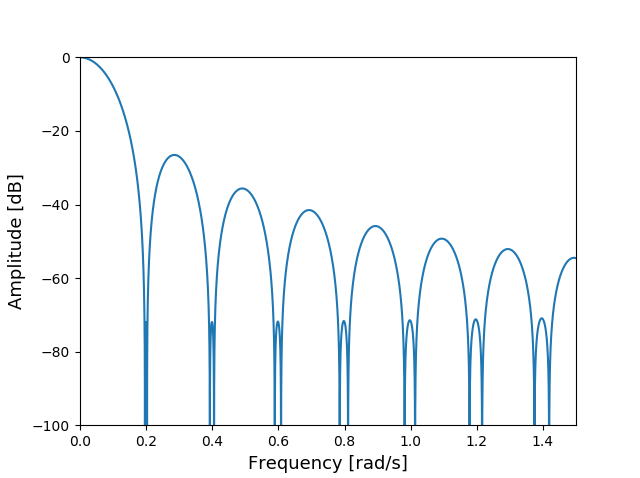
\includegraphics[width=\textwidth]{figures/dbplots/stft_bilag/64/bartlett.png}
\caption{Bartlett window.}
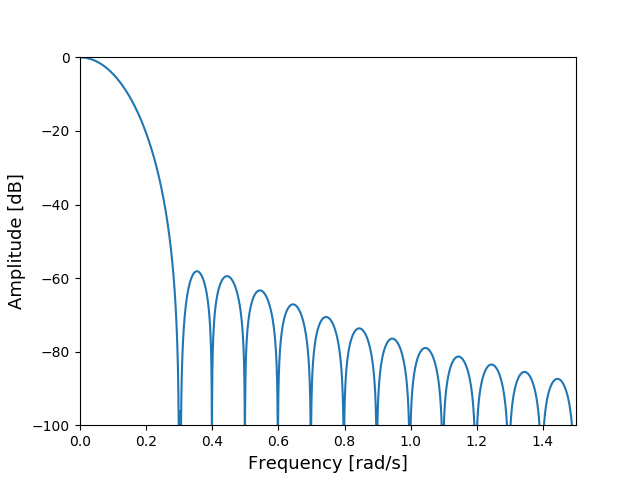
\includegraphics[width=\textwidth]{figures/dbplots/stft_bilag/64/blackman.png}
\caption{Blackman window.}
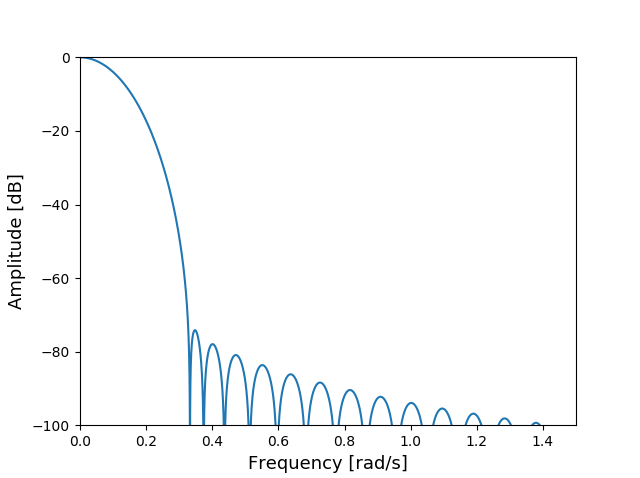
\includegraphics[width=\textwidth]{figures/dbplots/stft_bilag/64/kaiser10.png}
\caption{Kaiser window, $\beta=10$.}
\end{subfigure}

\caption{Amplitude responses in dB of window functions of order $M=64$.}
\label{fig:db_plots_64}
\end{figure}

\begin{figure}[H]
\centering

\begin{subfigure}{0.49\textwidth}
\centering
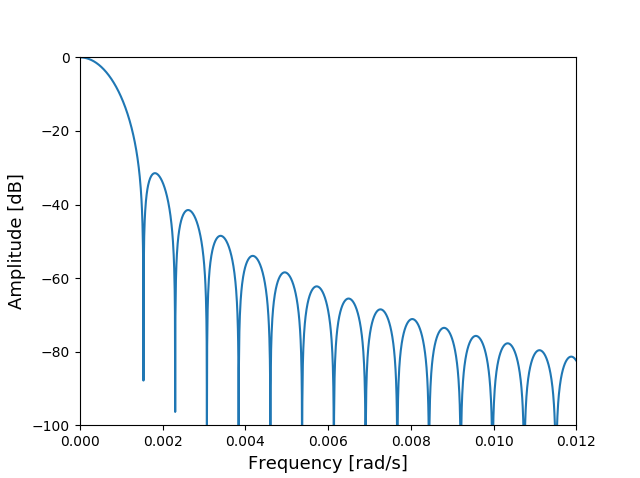
\includegraphics[width=\textwidth]{figures/dbplots/stft_bilag/8192/hann.png}
\caption{Hann window.}
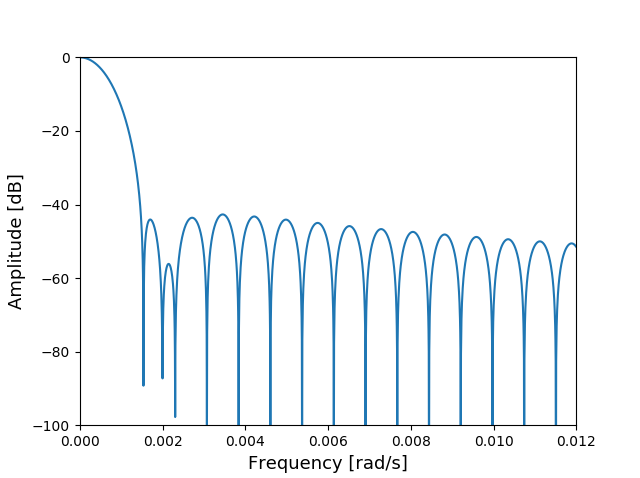
\includegraphics[width=\textwidth]{figures/dbplots/stft_bilag/8192/hamming.png}
\caption{Hamming window.}
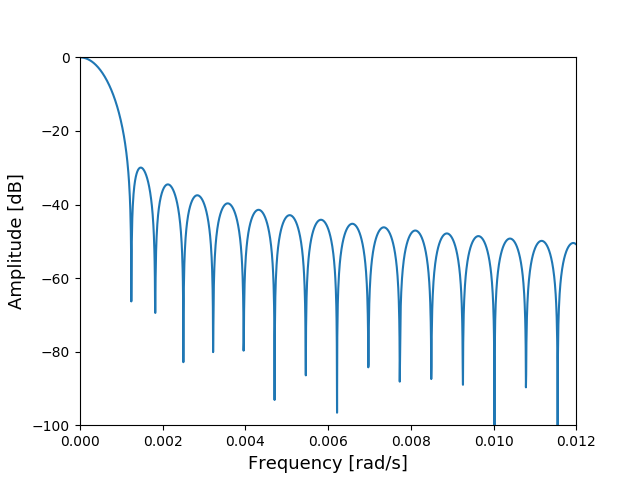
\includegraphics[width=\textwidth]{figures/dbplots/stft_bilag/8192/kaiser4.png}
\caption{Kaiser window, $\beta=4$.}
\end{subfigure}
\centering
\begin{subfigure}{0.49\textwidth}
\centering
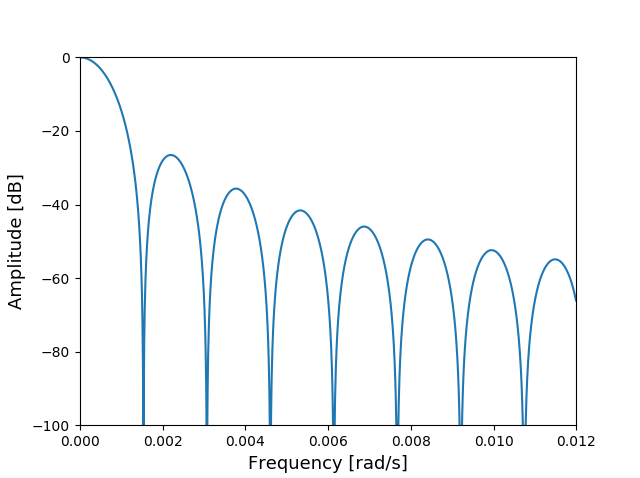
\includegraphics[width=\textwidth]{figures/dbplots/stft_bilag/8192/bartlett.png}
\caption{Bartlett window.}
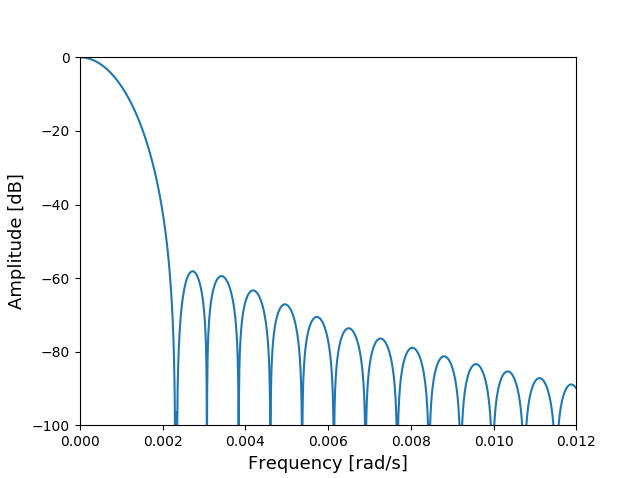
\includegraphics[width=\textwidth]{figures/dbplots/stft_bilag/8192/blackman.png}
\caption{Blackman window.}
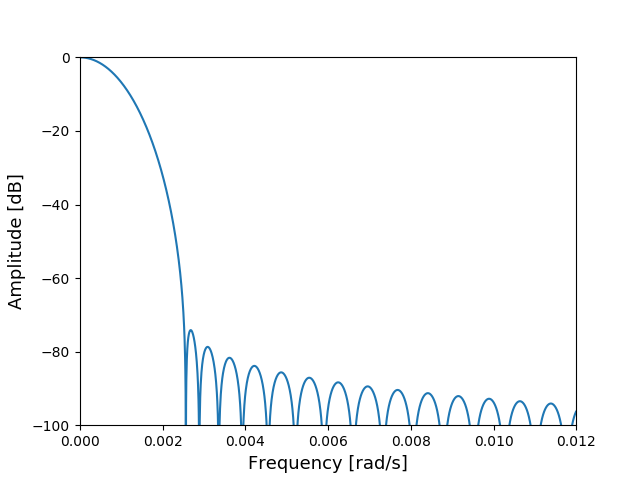
\includegraphics[width=\textwidth]{figures/dbplots/stft_bilag/8192/kaiser10.png}
\caption{Kaiser window, $\beta=10$.}
\end{subfigure}

\caption{Amplitude responses in dB of window functions of order $M=8192$.}
\label{fig:db_plots_8192}
\end{figure}